\section{Технологический раздел}
В этом разделе будет проведен выбор средств реализации ПО.
Будет выбран язык программирования, система управления базой данных, ПО для графического интерфейса.
Будут приведены листинги кода для реализованной базы данных и листинги реализации взаимодействия приложения и базы данных.
Будет проведена демонстрация работы программы с реализованным функционалом для каждой роли.

\subsection{Средства реализации программного обеспечения}
\subsubsection{Выбор языка программирования}
В качестве языка программирования для реализации платформы был выбран Python 3.9, так как имеется опыт разработки проектов на этом языке. 
Также данный язык программирования поддерживает парадигму ООП, соответственно, даёт возможность реализовать структуру приложения, приведённую в конструкторской части.
В качестве библиотеки для реализации взаимодействия приложения и базы данных была выбрана psycopg \cite{psycopg2}, так как автор имеет опыт работы с этой библиотекой.

\subsubsection{Выбор СУБД}
В качестве СУБД был выбран PostgreSQL.

Postgres \cite{postgresql} -- это свободно распространяемая объектно-реляционная система управления базами данных.
Данная СУБД предназначена для обработки ряда рабочих нагрузок, от отдельных компьютеров до хранилищ данных или веб-сервисов с множеством одновременных пользователей. 

Выбор обусловлен тем, что имеется опыт разработки проектов с данной СУБД, а также тем, что Python и PostgreSQL являются совместимыми технологиями  \cite{psycopg2}.

\subsubsection{Выбор ПО для графического интерфейса}
В качестве ПО для реализации UI был выбран среда QT по следующим причинам:
\begin{enumerate}
	\item Qt предоставляет широкую поддержку для взаимодействия с Python приложениями.
	\item Qt является программной средой для реализации Desktop-приложений. Пользователь может воспользоваться ПО QtDesigner для разработки UI.
	\item Структура приложений QT позволяет внедрить их в ООП-архитектуру.
	\item У автора есть опыт разработки проектов с использованием QT.
\end{enumerate} 

\subsection{Листинги кода}

\subsubsection{Создание базы данных}
В работе была реализована база данных, соответствующая разработанной в аналитическом и конструкторских разделах.
Помимо создания таблиц, требуется наложить на каждую ограничения.
Были добавлены следующие ограничения:
\begin{itemize}
	\item \textbf{Account} -- баланс игрока должен быть положительным, игроку должно быть не меньше 18 лет, номер паспорта должен состоять из 10 символов, без пробелов;
	\item \textbf{Games} -- корректные коэффициенты (больше 1), сумма вероятностей событий с учётом маржи не меньше, чем 1;
	\item \textbf{Bet} -- сумма ставки от 10 до 1000 у.е, коэффициент больше 1;
	\item \textbf{Users} -- логин и пароль должны состоять как минимум из 5 символов.
\end{itemize} 

Код создания всех таблиц в базе данных с указанием типов атрибутов представлен в приложении А.

Код создания ограничений на таблицы представлен в приложении Б.

\subsubsection{Функции, хранимые процедуры и триггеры}
Всего в работе было реализовано 10 функций и 11 процедур.

В списке перечислены реализованные процедуры и функции:
\begin{itemize}
	\item \textbf{BK.viewTeams(myTeamName text)} -- функция, возвращает команды, доступные для добавления в матч;
	\item \textbf{BK.verifyAccs(surnameString text)} -- функция, возвращает список аккаунтов, которые ждут аутентификации. Аргумент функции соответствует фамилии, по которой требуется производить поиск;
	\item \textbf{BK.getUserInfo(webUserLog text)} -- функция, возвращает полную информацию об пользователе;
	\item \textbf{BK.auth(login text, password text)} -- функция, проверяющая, есть ли аккаунт с логином и паролем в процессе авторизации;
	\item \textbf{BK.findLogin(login text)} -- функция, проверяющая наличие логина в таблице Account;
	\item \textbf{BK.viewGamesAnalyze(name text)} -- функция, возвращающая актуальную линию событий;
	\item \textbf{BK.GetResult(id int)} -- функция, возвращающая победителя матча;
	\item \textbf{BK.GetBetHistory(id int)} -- функция, возвращающая историю ставок по пользователю;
	\item \textbf{BK.GetROI(id int)} -- функция, возвращающая общую доходность пользователя;
	\item \textbf{BK.GetAllActiveAccs()} -- функция, которая возвращает все активные аккаунты в системе;
	\item \textbf{BK.insertUsers(args)} -- процедура, которая добавляет пользователя в таблицу Users;
	\item \textbf{BK.insertAccount(args)} -- процедура добавления нового игрока в таблицу Account;
	\item \textbf{BK.registrate(args)} -- процедура регистрации игрока в систему;
	\item \textbf{BK.updateStatus(id int, status text)} -- процедура изменения статуса аккаунта;
	\item \textbf{BK.addGame(args)} -- процедура добавления нового матча в систему;
	\item \textbf{BK.changeGameState(id int)} -- процедура изменения статуса матча;
	\item \textbf{BK.changeGameResult(id int, result text)} -- процедура изменения счёта матча;
	\item \textbf{BK.changeGameCoef(args)} -- процедура изменения коэффициентов для конкретного матча;
	\item \textbf{BK.MakeBet(args)} -- процедура совершения ставки;
	\item \textbf{BK.Donate(id INT, value float)} -- процедура пополнения баланса игроком.
	\item \textbf{BK.UpdateBalance(id int)} -- процедура платежа клиентам выигранной суммы после завершения матча.
\end{itemize}

\newpage
На листинге 1 представлен код получения таблицы матчей в текущей линии:
\FloatBarrier
\begin{lstinputlisting}[language=SQL, caption=Получение таблицы матчей в текущей линии, linerange = {78-101},
	basicstyle=\footnotesize\ttfamily, frame=single, breaklines=true]{src/db/sql/functions.sql}
\end{lstinputlisting}
\FloatBarrier

\newpage
На листинге 2 представлен код расчёта итога события:
\FloatBarrier
\begin{lstinputlisting}[language=SQL, caption=Расчёт итога события, linerange = {127-151},
	basicstyle=\footnotesize\ttfamily, frame=single,breaklines=true]{src/db/sql/functions.sql}
\end{lstinputlisting}
\FloatBarrier

\subsubsection{Триггеры}
Триггеры в программе позволяют автоматизировать процесс денежных выплат при выполнении ставки игроком и при расчёте выплаты игрокам по окончанию события.

Было разработано два триггера:
\begin{enumerate}
	\item \textbf{BK.MakeBet()} -- триггер, который списывает с баланса игрока сумму, равную размеру ставки, при заключении пари с БК. Триггер обновляет таблицу Account при добавлении новой записи в таблицу Bet.
	\item \textbf{BK.UpdateBet()} -- триггер, который обновляет баланс всех игроков, которые ставили на только что завершённое событие. Триггер обновляет таблицы Account и Bet при изменении таблицы Games.
\end{enumerate}

На листинге 3 представлен код триггера UpdateBet, связанным с изменением состояния матча:
\FloatBarrier
\begin{lstinputlisting}[language=SQL, caption=Триггер на обновление таблицы Games, linerange = {24-50},
	basicstyle=\footnotesize\ttfamily, frame=single,breaklines=true]{src/db/sql/triggers.sql}
\end{lstinputlisting}
\FloatBarrier

\newpage
На листинге 4 представлен код процедуры обновления баланса пользователей BK.UpdateBalance(id int), которая вызывается внутри триггера UpdateBet:
\FloatBarrier
\begin{lstinputlisting}[language=SQL, caption=Обновление балансов пользователй, linerange = {112-134},
	basicstyle=\footnotesize\ttfamily, frame=single,breaklines=true]{src/db/sql/procedures.sql}
\end{lstinputlisting}
\FloatBarrier

\newpage
\subsubsection{Ролевая модель на уровне БД}
В соответствии с ролевой моделью, были созданы следующие роли:
\begin{enumerate}
	\item \textbf{Client} -- роль, связанная с игроком. Игрок обладает правами на доступ к таблице матчей и ставок, так как он должен совершать ставки и видеть список матчей.
	\item \textbf{Administrator} -- роль, связанная с администратором. Ему выданы полные права на таблицы Users, Account и Bet. Наличие последней обусловлено тем, что администратор имеет возможность увидеть доходность активных пользователей, чтобы заблокировать прибыльных игроков.
	\item \textbf{Analyzist} -- роль, связанная с аналитиком. Он обладает доступом к таблицам Teams, Games и Bet.
\end{enumerate}

На листинге 5 представлен код выдачи прав по ролям:
\FloatBarrier
\begin{lstinputlisting}[language=SQL, caption=Выдача прав ролям, 
	basicstyle=\footnotesize\ttfamily, frame=single,breaklines=true]{src/db/sql/roles.sql}
\end{lstinputlisting}
\FloatBarrier

\newpage
\subsubsection{Приложение}
Все действия, которые приложение может выполнить, обернуты в SQL функции, которые затем вызываются классами, ответственными за взаимодействие с базой данных.

На листинге 6 представлен код выполнения SQL-запроса в Python:
\FloatBarrier
\begin{lstinputlisting}[language=Python, caption=Выполнение SQL-запроса, linerange = {11-28},
	basicstyle=\footnotesize\ttfamily, frame=single,breaklines=true]{src/db/baseRepo.py}
\end{lstinputlisting}
\FloatBarrier

На листинге 7 представлен код пополнения баланса пользователя:
\FloatBarrier
\begin{lstinputlisting}[language=Python, caption=Пополнение баланса пользователя, linerange = {44-47},
	basicstyle=\footnotesize\ttfamily, frame=single,breaklines=true]{src/db/playerRepo.py}
\end{lstinputlisting}
\FloatBarrier

\newpage
\subsection{Демонстрация работы программы}
В этом разделе будут показана демонстрация работы программы при выполнении основных действий для каждой из представленных в программе ролей. Будет рассмотрена авторизация в системе, регистрация нового игрока, процесс создания нового матча и изменения коэффициентов для аналитика, процесс верификации аккаунтов для администратора, и процессы работы с БК для игрока.

\subsubsection{Вход в систему}
Стартовый экран приложения представлен на рисунке \ref{fig::start}. 
Пользователь может войти в систему, введя логин и пароль в специальных полях ввода.
При успешной авторизации пользователь перейдёт в следующее окно, которое соответствует его роли.
Ввод логина и пароля чувствителен к регистру.
Также отсюда можно перейти к регистрации, нажав на кнопку «Регистрация». 

\FloatBarrier
\begin{figure}[hp]	
	\begin{center}
		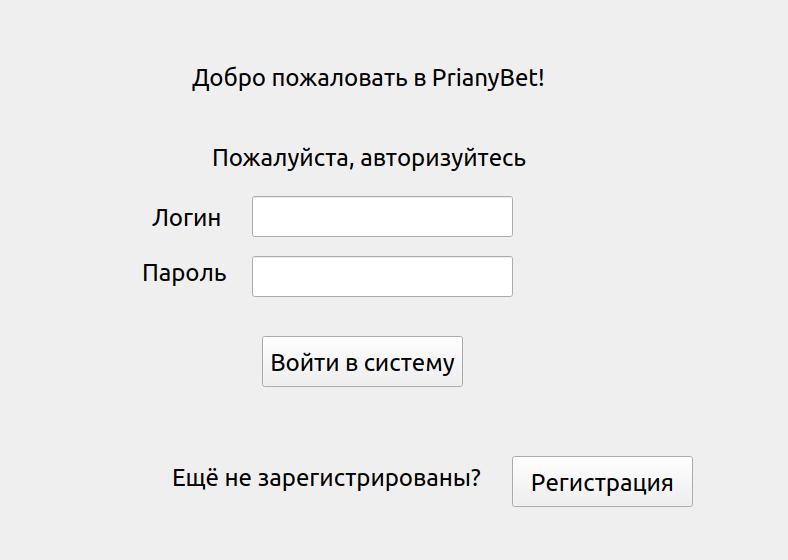
\includegraphics[width=\linewidth]{inc/start.png}
	\end{center}
	\captionsetup{justification=centering, labelsep=defffis}
	\caption{Стартовый экран приложения}
	\label{fig::start}
\end{figure}
\FloatBarrier

\newpage
\subsubsection{Регистрация}
Экран регистрации представлен на рисунке \ref{fig::reg}. 
Пользователь вводит все данные, которые после ввода проверяются программой.
Игроку не должно быть меньше 18 лет, почта должна быть указана корректно.
Для указания номера телефона позволительно использовать префикс + или же начинать номер с 8.
Длина паспорта должна быть 10 символов, серия и номер пишутся слитно.
В случае успеха пользователь регистрируется в системе, либо же система выведет сообщение об ошибке.

\FloatBarrier
\begin{figure}[hp]	
	\begin{center}
		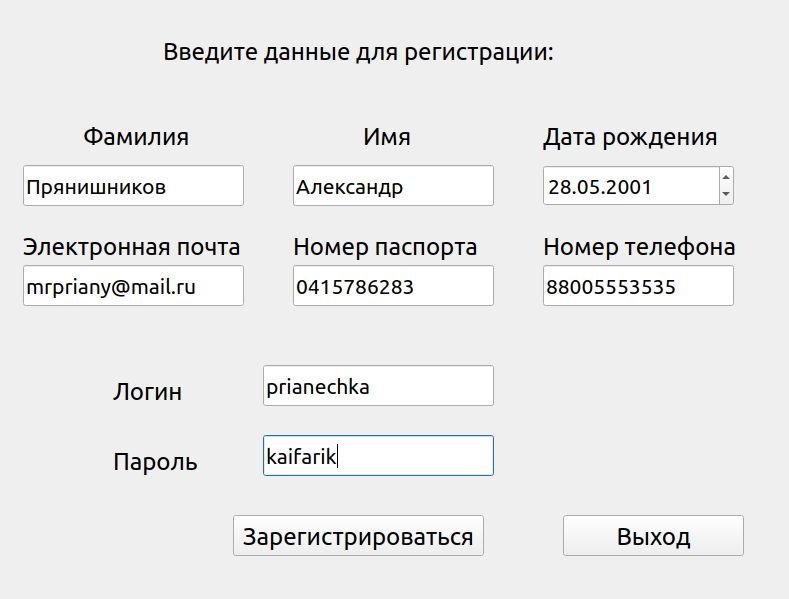
\includegraphics[width=\linewidth]{inc/registrate.png}
	\end{center}
	\captionsetup{justification=centering, labelsep=defffis}
	\caption{Экран регистрации}
	\label{fig::reg}
\end{figure}
\FloatBarrier

\newpage
\subsubsection{Стартовое меню игрока}
Стартовый экран игрока представлен на рисунке \ref{fig::user}. 
Игрок может посмотреть сверху свои данные: баланс, логин, а также статус аккаунта.
В случае, если игрок не обладает статусом «Активен», то кнопки «История ставок», «Пополнить баланс» и «Ставить!» будут недоступны.
С этого экрана можно перейти к просмотру истории ставок, пополнению баланса или непосредственно к выполнению ставок.

\FloatBarrier
\begin{figure}[h]	
	\begin{center}
		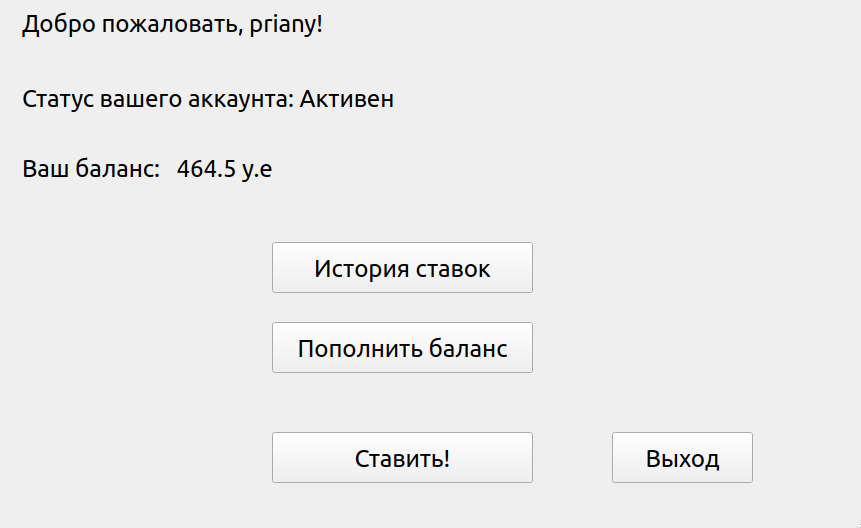
\includegraphics[width=\linewidth]{inc/user.png}
	\end{center}
	\captionsetup{justification=centering, labelsep=defffis}
	\caption{Стартовый экран игрока}
	\label{fig::user}
\end{figure}
\FloatBarrier

\subsubsection{Пополнение баланса}
Экран пополнения баланса представлен на рисунке \ref{fig::balance}. 
Игрок выбирает сумму пополнения, после чего при нажатии кнопки «Пополнить баланс» баланс успешно пополняется. 
В случае успешного пополнения игрок увидит графическое уведомление о том, что деньги пришли на счёт.
Также из этого экрана можно перейти в главное меню игрока, нажав на кнопку «Выход». 
Сумма пополнения ограничена суммой 1000 у.е. 

\FloatBarrier
\begin{figure}[h]	
	\begin{center}
		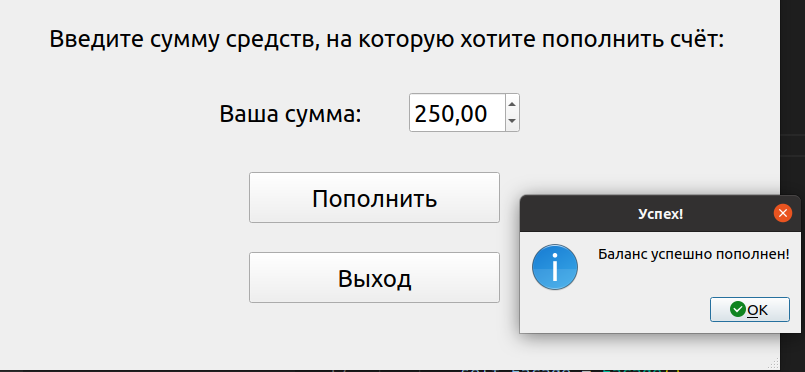
\includegraphics[height = 6cm, width=\linewidth]{inc/balance.png}
	\end{center}
	\captionsetup{justification=centering, labelsep=defffis}
	\caption{Экран пополнения баланса}
	\label{fig::balance}
\end{figure}
\FloatBarrier

\subsubsection{Выполнение ставок}
Экран выполнения ставок представлен на рисунке \ref{fig::bet}.

Игрок может увидеть в таблице все события, которые присутствуют в линии в данный момент.
Для выбора события, на которое нужно сделать ставку, пользователь должен выделить строку с нужным событием.
Слева внизу игрок может выбрать событие для ставки, а также сумму, на которую он хочет заключить пари.

После нажатия кнопки выполнения ставки программа оценит валидность введённых данных, и, в случае успеха, выдаст информационное сообщение.

\FloatBarrier
\begin{figure}[h]	
	\begin{center}
		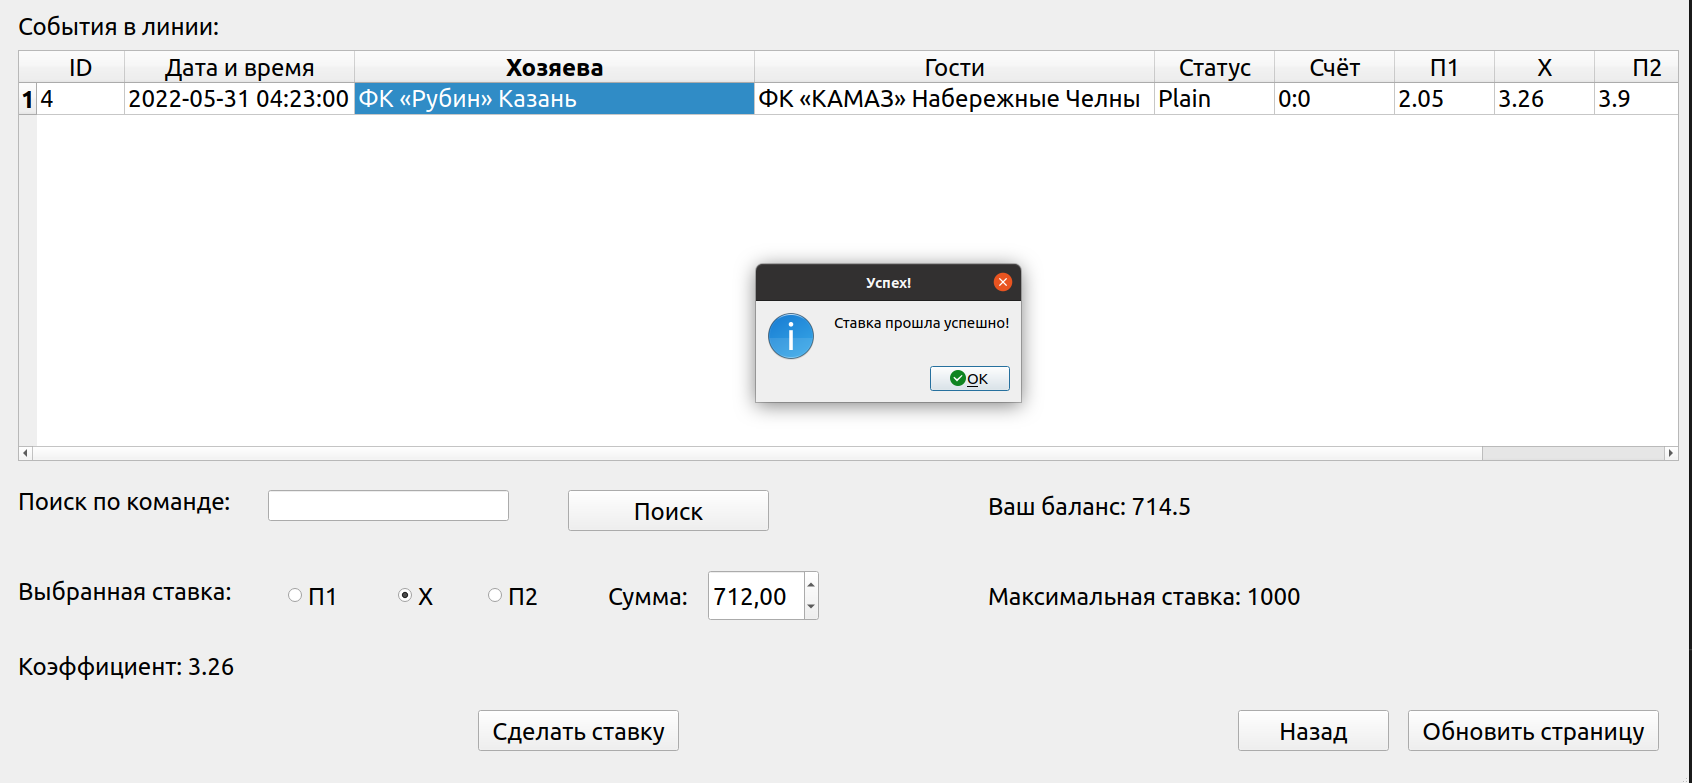
\includegraphics[height = 7cm, width=\linewidth]{inc/bet.png}
	\end{center}
	\captionsetup{justification=centering, labelsep=defffis}
	\caption{Экран выполнения ставок}
	\label{fig::bet}
\end{figure}
\FloatBarrier

\subsubsection{Просмотр истории ставок}
Экран просмотра истории ставок представлен на рисунке \ref{fig::history}.

Игрок может увидеть в таблице все события, которые присутствуют в линии в данный момент.
Для выбора события, на которое нужно сделать ставку, пользователь должен выделить строку с нужным событием.
Слева внизу игрок может выбрать событие для ставки, а также сумму ставки.

После нажатия кнопки выполнения ставки программа оценит валидность введённых данных, и, в случае успеха, выдаст информационное сообщение.

\FloatBarrier
\begin{figure}[h]	
	\begin{center}
		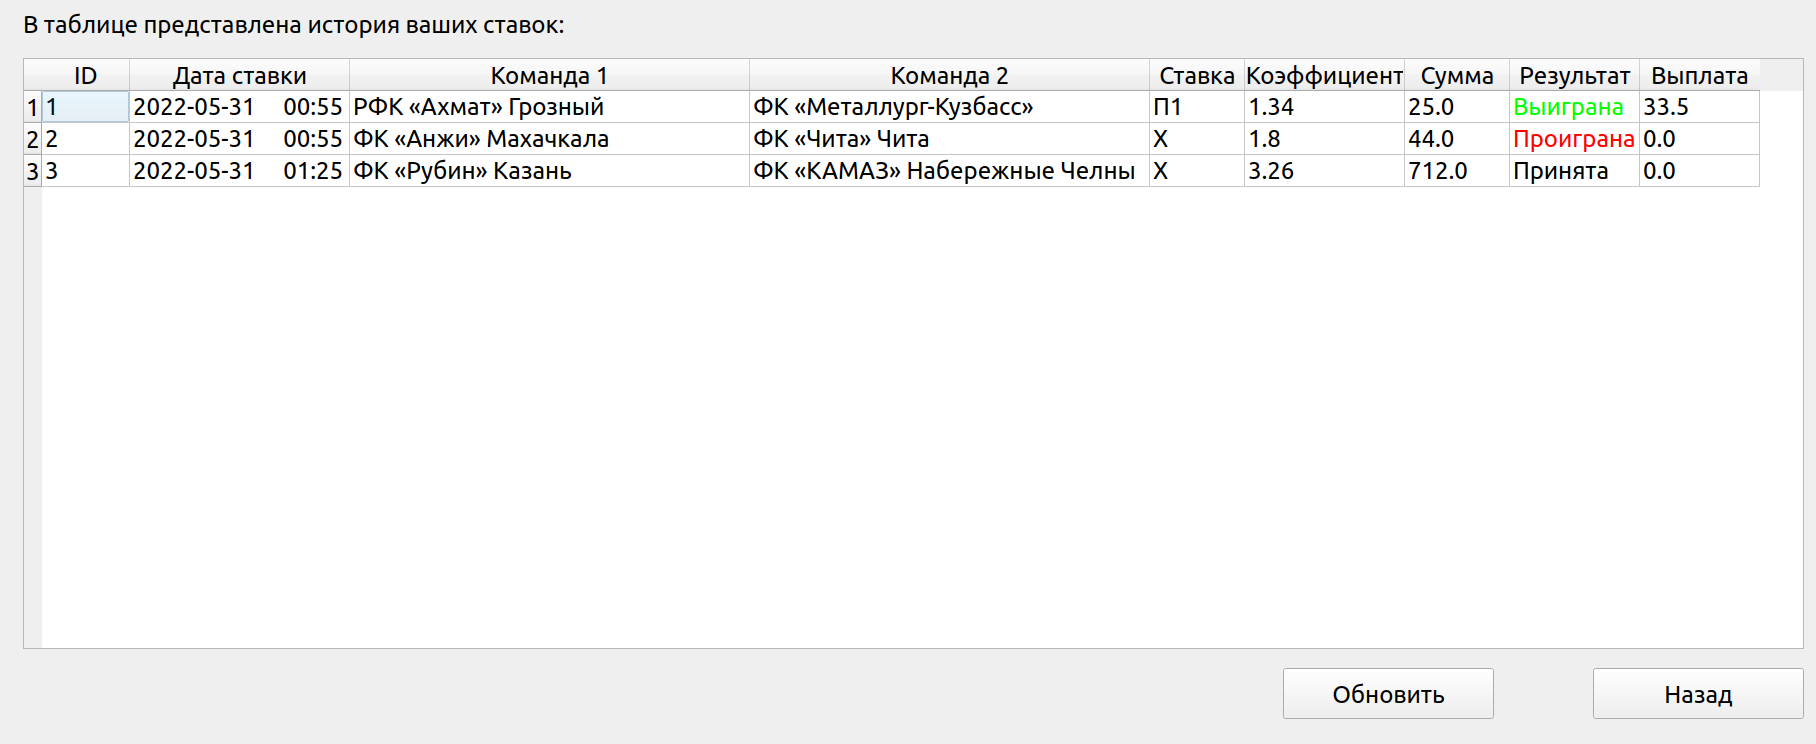
\includegraphics[width=\linewidth]{inc/history.png}
	\end{center}
	\captionsetup{justification=centering, labelsep=defffis}
	\caption{Экран просмотра истории ставок}
	\label{fig::history}
\end{figure}
\FloatBarrier

\subsubsection{Добавление матчей в линию аналитиком}
Экран добавления матчей в линию представлен на рисунке \ref{fig::add}.

Экран доступен только в случае входа аналитика в приложение из стартового окна.
В таблице представлен список клубов, доступных для добавления в событие.
Можно воспользоваться кнопкой поиска для нахождения клубов.
Выбор команды осуществляется нажатием на название мышкой.

Также внизу аналитик должен выбрать вероятности наступления событий. 
Сумма вероятностей должна быть равна 100\%.

\FloatBarrier
\begin{figure}[h]	
	\begin{center}
		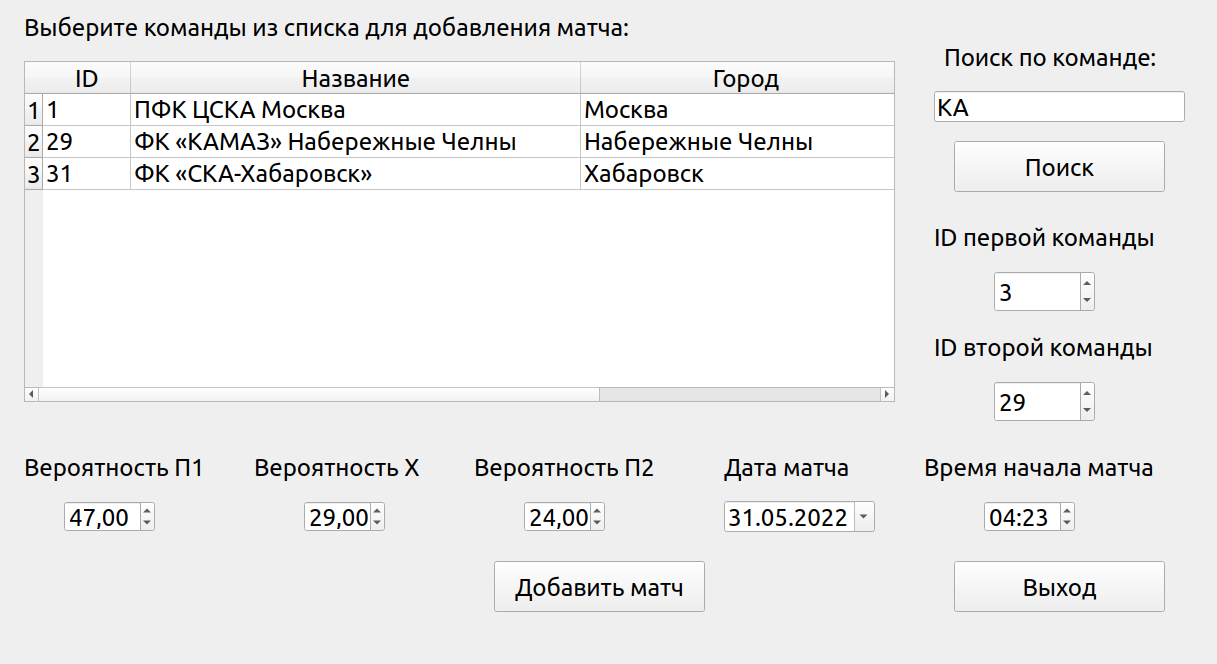
\includegraphics[width=\linewidth]{inc/addMatch.png}
	\end{center}
	\captionsetup{justification=centering, labelsep=defffis}
	\caption{Экран добавления матчей в линию}
	\label{fig::add}
\end{figure}
\FloatBarrier

\subsubsection{Экран изменения матчей}
Экран изменения матчей в линии представлен на рисунке \ref{fig::change}.

Экран доступен только в случае входа аналитика в приложение из стартового окна.
В таблице представлены матчи, добавленные аналитиком в предыдущем окне.
Для изменения состояния матча или изменения счёта нужно нажать на строку с событием, а затем нажать на требуемую кнопку внизу таблицы.

Также внизу аналитик может изменить вероятности наступления событий.

\FloatBarrier
\begin{figure}[h]	
	\begin{center}
		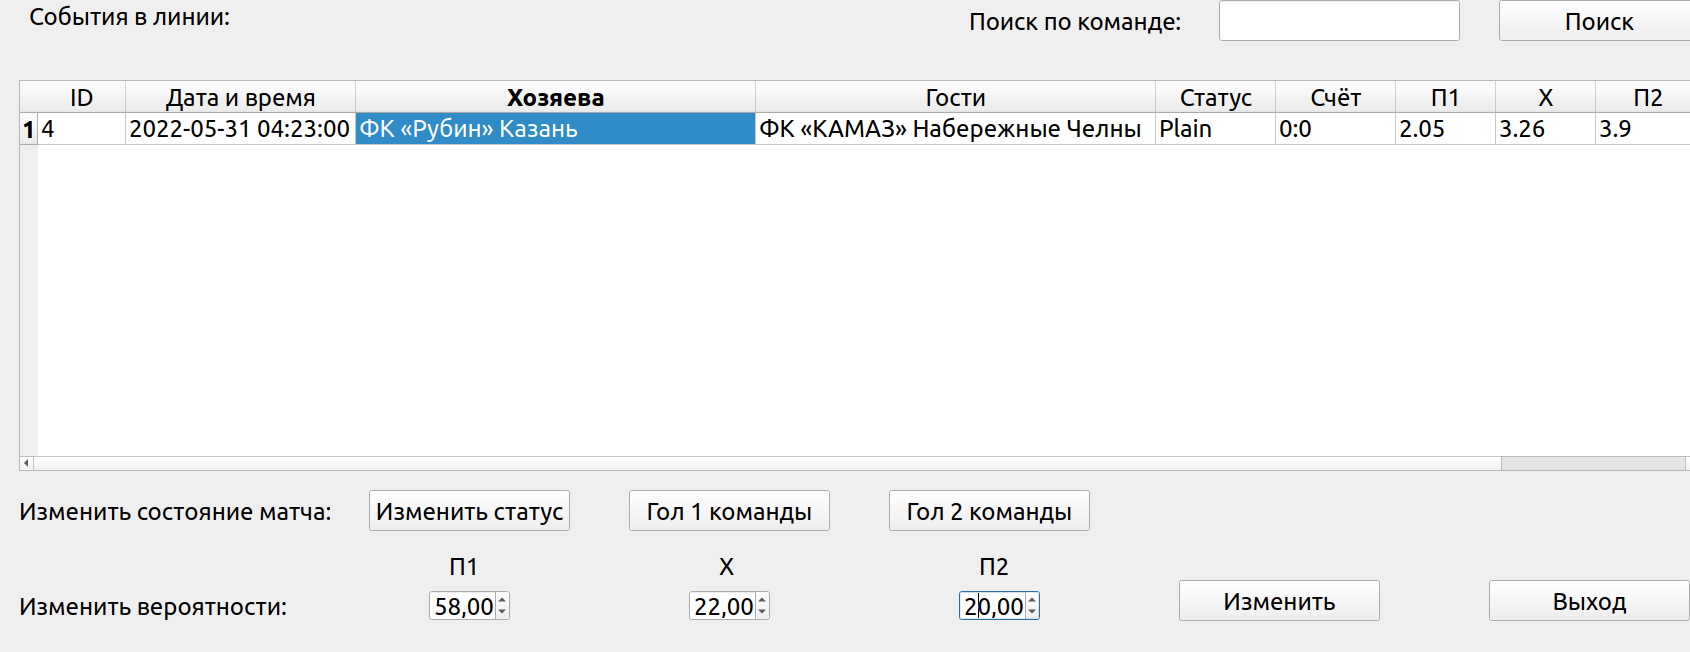
\includegraphics[height=6cm, width=\linewidth]{inc/matches.png}
	\end{center}
	\captionsetup{justification=centering, labelsep=defffis}
	\caption{Экран изменения матчей в линию}
	\label{fig::change}
\end{figure}
\FloatBarrier

\subsubsection{Экран верификации пользователей}
Экран верификации пользователей в линии представлен на рисунке \ref{fig::verify}.

Экран доступен только в случае входа администратора в приложение из стартового окна.
Аналитик в таблице видит список аккаунтов, которые требуют верификации.
В зависимости от введённых данных аналитик может либо верифицировать аккаунт, либо заблокировать.

\FloatBarrier
\begin{figure}[h]	
	\begin{center}
		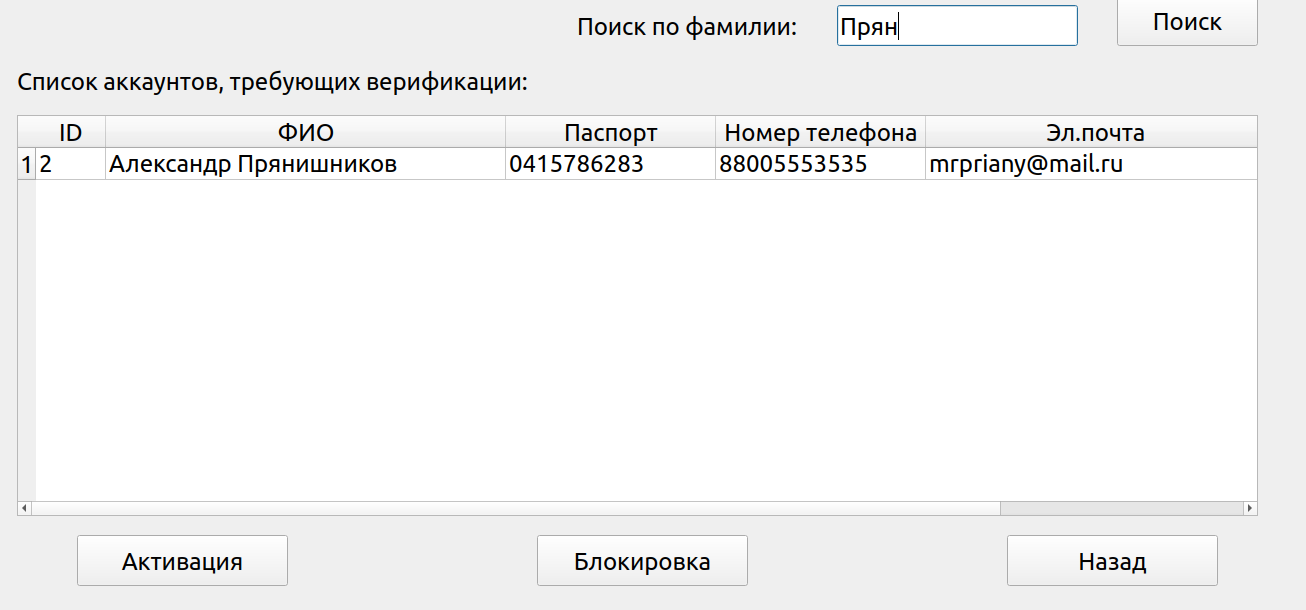
\includegraphics[width=\linewidth]{inc/verify.png}
	\end{center}
	\captionsetup{justification=centering, labelsep=defffis}
	\caption{Экран верификации пользователей}
	\label{fig::verify}
\end{figure}
\FloatBarrier